%%%%%%%%%%%%%%%%%%%%%%%%%%%%%%%%%%%%%%%%%%%%%%%%%%%%%%%%%%%%
% 5.2 SINGLE-VARIABLE CALCULUS
% The Composition of Advanced Mathematics
%%%%%%%%%%%%%%%%%%%%%%%%%%%%%%%%%%%%%%%%%%%%%%%%%%%%%%%%%%%%

\section{Single-Variable Calculus}
\label{sec:single-variable-calculus}

\prerequisite{
Precalculus and functions from \cref{sec:precalculus-functions},
elementary algebra from \cref{sec:elementary-algebra}, functions from
\cref{sec:functions}, and basic trigonometric, exponential, and logarithmic
function behavior developed in the preceding section.
}

\learningobjectives{
By the end of this section, the reader should be able to:
\begin{itemize}
    \item interpret limits numerically, graphically, and algebraically;
    \item distinguish one-sided, two-sided, infinite, and limits at infinity;
    \item apply limit laws and algebraic techniques for evaluating limits;
    \item define and analyze continuity;
    \item interpret the derivative as an instantaneous rate of change and
    tangent-line slope;
    \item compute derivatives using foundational differentiation rules;
    \item differentiate polynomial, rational, trigonometric, inverse
    trigonometric, exponential, and logarithmic functions;
    \item apply the chain rule and implicit differentiation;
    \item analyze increasing, decreasing, concavity, and extrema;
    \item solve optimization and related-rate problems;
    \item define antiderivatives and indefinite integrals;
    \item interpret definite integrals through signed area and accumulation;
    \item state and use the Fundamental Theorem of Calculus;
    \item apply substitution;
    \item compute area, average value, displacement, and volume using integrals;
    \item explain the conceptual relationship among limits, derivatives,
    and integrals.
\end{itemize}
}

%%%%%%%%%%%%%%%%%%%%%%%%%%%%%%%%%%%%%%%%%%%%%%%%%%%%%%%%%%%%
\subsection{The Central Ideas of Calculus}
\label{subsec:central-ideas-calculus}
%%%%%%%%%%%%%%%%%%%%%%%%%%%%%%%%%%%%%%%%%%%%%%%%%%%%%%%%%%%%

Single-variable calculus studies functions whose inputs and outputs are
typically real numbers.

Its two central problems are:

\begin{enumerate}
    \item determining instantaneous rates of change;
    \item determining accumulated quantities.
\end{enumerate}

These lead to derivatives and integrals.

Both are built from limits.

\begin{center}
\begin{tikzpicture}[
    node distance=11mm and 18mm,
    box/.style={draw,rounded corners,align=center,inner sep=6pt},
    >=stealth
]
\node[box] (limits) {Limits};
\node[box,below left=of limits] (deriv) {Derivatives\\instantaneous change};
\node[box,below right=of limits] (integ) {Integrals\\accumulation};
\node[box,below=18mm of $(deriv)!0.5!(integ)$] (ftc)
{Fundamental Theorem\\of Calculus};

\draw[->] (limits)--(deriv);
\draw[->] (limits)--(integ);
\draw[->] (deriv)--(ftc);
\draw[->] (integ)--(ftc);
\end{tikzpicture}
\end{center}

\begin{conceptbox}
Calculus is built around the idea of studying quantities through arbitrarily
small changes.

Limits make this precise.
\end{conceptbox}

%%%%%%%%%%%%%%%%%%%%%%%%%%%%%%%%%%%%%%%%%%%%%%%%%%%%%%%%%%%%
\subsection{Limits}
\label{subsec:limits-introduction}
%%%%%%%%%%%%%%%%%%%%%%%%%%%%%%%%%%%%%%%%%%%%%%%%%%%%%%%%%%%%

Consider a function \(f\) and a number \(a\).

The expression

\[ \lim_{x\to a}f(x)=L \]

is read:

``the limit of \(f(x)\) as \(x\) approaches \(a\) is \(L\).''

Here:

\begin{itemize}
    \item \(\lim\) means \emph{limit};
    \item \(x\to a\) means ``\(x\) approaches \(a\)'';
    \item \(L\) is the value approached by \(f(x)\).
\end{itemize}

The limit concerns the behavior of \(f(x)\) near \(a\), not necessarily the
value of \(f(a)\).

%%%%%%%%%%%%%%%%%%%%%%%%%%%%%%%%%%%%%%%%%%%%%%%%%%%%%%%%%%%%
\subsection{Graphical Interpretation of a Limit}
\label{subsec:graphical-limit}
%%%%%%%%%%%%%%%%%%%%%%%%%%%%%%%%%%%%%%%%%%%%%%%%%%%%%%%%%%%%

Suppose a graph approaches the height \(L\) as \(x\) approaches \(a\) from
both sides.

Then

\[ \lim_{x\to a}f(x)=L. \]

The value \(f(a)\) may:

\begin{itemize}
    \item equal \(L\);
    \item differ from \(L\);
    \item fail to exist.
\end{itemize}

The limit depends on nearby behavior.

%%%%%%%%%%%%%%%%%%%%%%%%%%%%%%%%%%%%%%%%%%%%%%%%%%%%%%%%%%%%
\subsection{A Limit with a Hole}
\label{subsec:limit-hole}
%%%%%%%%%%%%%%%%%%%%%%%%%%%%%%%%%%%%%%%%%%%%%%%%%%%%%%%%%%%%

Consider

\[ f(x)=\frac{x^2-4}{x-2}. \]

For \(x\neq2\),

\[ f(x)=x+2. \]

Although \(f(2)\) is undefined, nearby values approach \(4\).

Therefore,

\[ \boxed{\lim_{x\to2}\frac{x^2-4}{x-2}=4.} \]

This illustrates why a limit is not simply substitution.

%%%%%%%%%%%%%%%%%%%%%%%%%%%%%%%%%%%%%%%%%%%%%%%%%%%%%%%%%%%%
\subsection{One-Sided Limits}
\label{subsec:one-sided-limits}
%%%%%%%%%%%%%%%%%%%%%%%%%%%%%%%%%%%%%%%%%%%%%%%%%%%%%%%%%%%%

Sometimes a function behaves differently on the two sides of a point.

The left-hand limit is written

\[ \lim_{x\to a^-}f(x). \]

The superscript minus sign indicates that \(x\) approaches \(a\) from values
less than \(a\).

The expression is read:

``the limit of \(f(x)\) as \(x\) approaches \(a\) from the left.''

The right-hand limit is

\[ \lim_{x\to a^+}f(x), \]

read:

``the limit of \(f(x)\) as \(x\) approaches \(a\) from the right.''

%%%%%%%%%%%%%%%%%%%%%%%%%%%%%%%%%%%%%%%%%%%%%%%%%%%%%%%%%%%%
\subsection{Two-Sided Limit Criterion}
\label{subsec:two-sided-limit-criterion}
%%%%%%%%%%%%%%%%%%%%%%%%%%%%%%%%%%%%%%%%%%%%%%%%%%%%%%%%%%%%

\begin{theorem}
The limit
\[ \lim_{x\to a}f(x)=L \]
exists if and only if
\[ \lim_{x\to a^-}f(x)=L
\qquad\text{and}\qquad
\lim_{x\to a^+}f(x)=L. \]
\end{theorem}

If the one-sided limits exist but are unequal, then the two-sided limit does
not exist.

%%%%%%%%%%%%%%%%%%%%%%%%%%%%%%%%%%%%%%%%%%%%%%%%%%%%%%%%%%%%
\subsection{Worked Example: One-Sided Limits}
\label{subsec:worked-one-sided-limits}
%%%%%%%%%%%%%%%%%%%%%%%%%%%%%%%%%%%%%%%%%%%%%%%%%%%%%%%%%%%%

\begin{workedexamplebox}{A Piecewise Limit}

Let

\[
f(x)=
\begin{cases}
x+1, & x<2,\\
5-x, & x\geq2.
\end{cases}
\]

Determine \(\lim_{x\to2}f(x)\).

\begin{tabularx}{\textwidth}{@{}>{\raggedright\arraybackslash}p{0.42\textwidth}X@{}}
Approach from the left using \(x+1\). &
\(\displaystyle \lim_{x\to2^-}f(x)=3\)\\
Approach from the right using \(5-x\). &
\(\displaystyle \lim_{x\to2^+}f(x)=3\)\\
The one-sided limits agree. &
\(\displaystyle \lim_{x\to2}f(x)=3\)
\end{tabularx}

\begin{answerbox}
\[ \boxed{\lim_{x\to2}f(x)=3.} \]
\end{answerbox}
\end{workedexamplebox}

%%%%%%%%%%%%%%%%%%%%%%%%%%%%%%%%%%%%%%%%%%%%%%%%%%%%%%%%%%%%
\subsection{When Limits Fail to Exist}
\label{subsec:limits-dne}
%%%%%%%%%%%%%%%%%%%%%%%%%%%%%%%%%%%%%%%%%%%%%%%%%%%%%%%%%%%%

A finite two-sided limit may fail to exist for several reasons.

Common examples include:

\begin{itemize}
    \item unequal one-sided limits;
    \item unbounded behavior;
    \item persistent oscillation;
    \item insufficiently stable local behavior.
\end{itemize}

For example,

\[
f(x)=
\begin{cases}
-1, & x<0,\\
1, & x\geq0
\end{cases}
\]

has

\[ \lim_{x\to0^-}f(x)=-1,\qquad
\lim_{x\to0^+}f(x)=1. \]

Therefore,

\[ \lim_{x\to0}f(x) \]

does not exist.

%%%%%%%%%%%%%%%%%%%%%%%%%%%%%%%%%%%%%%%%%%%%%%%%%%%%%%%%%%%%
\subsection{Limit Laws}
\label{subsec:limit-laws}
%%%%%%%%%%%%%%%%%%%%%%%%%%%%%%%%%%%%%%%%%%%%%%%%%%%%%%%%%%%%

Suppose

\[ \lim_{x\to a}f(x)=L,\qquad
\lim_{x\to a}g(x)=M. \]

Then, when the expressions are defined,

\[ \lim_{x\to a}[f(x)+g(x)]=L+M, \]

\[ \lim_{x\to a}[f(x)-g(x)]=L-M, \]

\[ \lim_{x\to a}f(x)g(x)=LM, \]

\[ \lim_{x\to a}cf(x)=cL, \]

and if \(M\neq0\),

\[ \lim_{x\to a}\frac{f(x)}{g(x)}=\frac{L}{M}. \]

Powers and roots may also be passed through limits under appropriate domain
conditions.

%%%%%%%%%%%%%%%%%%%%%%%%%%%%%%%%%%%%%%%%%%%%%%%%%%%%%%%%%%%%
\subsection{Direct Substitution}
\label{subsec:direct-substitution-limits}
%%%%%%%%%%%%%%%%%%%%%%%%%%%%%%%%%%%%%%%%%%%%%%%%%%%%%%%%%%%%

For many familiar continuous functions,

\[ \lim_{x\to a}f(x)=f(a). \]

Thus direct substitution is the first technique to try.

For example,

\[ \lim_{x\to3}(x^2-2x+4)
=3^2-2(3)+4=7. \]

%%%%%%%%%%%%%%%%%%%%%%%%%%%%%%%%%%%%%%%%%%%%%%%%%%%%%%%%%%%%
\subsection{Indeterminate Forms}
\label{subsec:indeterminate-forms-intro}
%%%%%%%%%%%%%%%%%%%%%%%%%%%%%%%%%%%%%%%%%%%%%%%%%%%%%%%%%%%%

Direct substitution sometimes produces expressions such as

\[ \frac00. \]

This is called an \emph{indeterminate form}.

It does not mean the limit equals zero or that the limit does not exist.

Instead, it signals that more analysis is required.

Other important indeterminate forms include

\[ \frac{\infty}{\infty},\qquad
0\cdot\infty,\qquad
\infty-\infty,\qquad
1^\infty,\qquad
0^0,\qquad
\infty^0. \]

Their rigorous treatment depends on context.

%%%%%%%%%%%%%%%%%%%%%%%%%%%%%%%%%%%%%%%%%%%%%%%%%%%%%%%%%%%%
\subsection{Factoring to Evaluate Limits}
\label{subsec:factoring-limits}
%%%%%%%%%%%%%%%%%%%%%%%%%%%%%%%%%%%%%%%%%%%%%%%%%%%%%%%%%%%%

Consider

\[ \lim_{x\to3}\frac{x^2-9}{x-3}. \]

Direct substitution gives

\[ \frac00. \]

Factor:

\[ x^2-9=(x-3)(x+3). \]

For \(x\neq3\),

\[ \frac{x^2-9}{x-3}=x+3. \]

Therefore,

\[ \boxed{\lim_{x\to3}\frac{x^2-9}{x-3}=6.} \]

%%%%%%%%%%%%%%%%%%%%%%%%%%%%%%%%%%%%%%%%%%%%%%%%%%%%%%%%%%%%
\subsection{Rationalizing Limits}
\label{subsec:rationalizing-limits}
%%%%%%%%%%%%%%%%%%%%%%%%%%%%%%%%%%%%%%%%%%%%%%%%%%%%%%%%%%%%

Radical expressions may require multiplication by a conjugate.

Consider

\[ \lim_{x\to0}\frac{\sqrt{x+1}-1}{x}. \]

Multiply by the conjugate:

\[
\frac{\sqrt{x+1}-1}{x}
\cdot
\frac{\sqrt{x+1}+1}{\sqrt{x+1}+1}
=
\frac{1}{\sqrt{x+1}+1}.
\]

Therefore,

\[ \boxed{\lim_{x\to0}\frac{\sqrt{x+1}-1}{x}=\frac12.} \]

%%%%%%%%%%%%%%%%%%%%%%%%%%%%%%%%%%%%%%%%%%%%%%%%%%%%%%%%%%%%
\subsection{The Squeeze Theorem}
\label{subsec:squeeze-theorem}
%%%%%%%%%%%%%%%%%%%%%%%%%%%%%%%%%%%%%%%%%%%%%%%%%%%%%%%%%%%%

\begin{theorem}[Squeeze Theorem]
Suppose
\[ g(x)\leq f(x)\leq h(x) \]
for all \(x\) sufficiently close to \(a\), except possibly at \(a\), and
\[ \lim_{x\to a}g(x)
=
\lim_{x\to a}h(x)
=L. \]
Then
\[ \lim_{x\to a}f(x)=L. \]
\end{theorem}

The theorem is useful when a complicated function is trapped between two
simpler functions approaching the same value.

%%%%%%%%%%%%%%%%%%%%%%%%%%%%%%%%%%%%%%%%%%%%%%%%%%%%%%%%%%%%
\subsection{The Fundamental Trigonometric Limit}
\label{subsec:fundamental-trig-limit}
%%%%%%%%%%%%%%%%%%%%%%%%%%%%%%%%%%%%%%%%%%%%%%%%%%%%%%%%%%%%

One of the most important limits in calculus is

\[ \boxed{\lim_{x\to0}\frac{\sin x}{x}=1,} \]

where \(x\) is measured in radians.

From this one obtains

\[ \lim_{x\to0}\frac{1-\cos x}{x}=0. \]

These limits form the foundation of the derivative formulas for sine and
cosine.

%%%%%%%%%%%%%%%%%%%%%%%%%%%%%%%%%%%%%%%%%%%%%%%%%%%%%%%%%%%%
\subsection{Infinite Limits}
\label{subsec:infinite-limits}
%%%%%%%%%%%%%%%%%%%%%%%%%%%%%%%%%%%%%%%%%%%%%%%%%%%%%%%%%%%%

Suppose

\[ f(x)\to+\infty \]

as \(x\to a\).

One writes

\[ \lim_{x\to a}f(x)=+\infty. \]

This is read:

``the limit of \(f(x)\) as \(x\) approaches \(a\) is positive infinity.''

This does not mean infinity is a real number.

Instead, it describes unbounded growth.

For example,

\[ \lim_{x\to0^+}\frac1x=+\infty. \]

%%%%%%%%%%%%%%%%%%%%%%%%%%%%%%%%%%%%%%%%%%%%%%%%%%%%%%%%%%%%
\subsection{Vertical Asymptotes and Limits}
\label{subsec:vertical-asymptotes-limits}
%%%%%%%%%%%%%%%%%%%%%%%%%%%%%%%%%%%%%%%%%%%%%%%%%%%%%%%%%%%%

A vertical line

\[ x=a \]

is a vertical asymptote when the function becomes unbounded as \(x\)
approaches \(a\) from at least one side.

For

\[ f(x)=\frac1{x-2}, \]

we have

\[ \lim_{x\to2^-}f(x)=-\infty, \]

and

\[ \lim_{x\to2^+}f(x)=+\infty. \]

Thus

\[ x=2 \]

is a vertical asymptote.

%%%%%%%%%%%%%%%%%%%%%%%%%%%%%%%%%%%%%%%%%%%%%%%%%%%%%%%%%%%%
\subsection{Limits at Infinity}
\label{subsec:limits-at-infinity}
%%%%%%%%%%%%%%%%%%%%%%%%%%%%%%%%%%%%%%%%%%%%%%%%%%%%%%%%%%%%

The expression

\[ \lim_{x\to\infty}f(x)=L \]

describes the behavior of \(f(x)\) as \(x\) grows without bound.

Similarly,

\[ \lim_{x\to-\infty}f(x)=L \]

describes behavior for large negative inputs.

If either limit equals \(L\), then

\[ y=L \]

is a corresponding horizontal asymptote.

%%%%%%%%%%%%%%%%%%%%%%%%%%%%%%%%%%%%%%%%%%%%%%%%%%%%%%%%%%%%
\subsection{Rational Functions at Infinity}
\label{subsec:rational-limits-infinity}
%%%%%%%%%%%%%%%%%%%%%%%%%%%%%%%%%%%%%%%%%%%%%%%%%%%%%%%%%%%%

Consider

\[ f(x)=\frac{2x^2+1}{x^2-3x}. \]

Divide numerator and denominator by \(x^2\):

\[ f(x)=\frac{2+1/x^2}{1-3/x}. \]

As \(x\to\infty\),

\[ \frac1x\to0,\qquad \frac1{x^2}\to0. \]

Therefore,

\[ \boxed{\lim_{x\to\infty}f(x)=2.} \]

Hence \(y=2\) is a horizontal asymptote.

%%%%%%%%%%%%%%%%%%%%%%%%%%%%%%%%%%%%%%%%%%%%%%%%%%%%%%%%%%%%
\subsection{Continuity}
\label{subsec:continuity}
%%%%%%%%%%%%%%%%%%%%%%%%%%%%%%%%%%%%%%%%%%%%%%%%%%%%%%%%%%%%

Informally, a function is continuous if its graph can be drawn locally
without a break.

The mathematical definition combines three conditions.

\begin{definitionbox}{Continuity at a Point}
A function \(f\) is \emph{continuous at \(x=a\)} if:
\begin{enumerate}
    \item \(f(a)\) is defined;
    \item \(\lim_{x\to a}f(x)\) exists;
    \item
    \[ \lim_{x\to a}f(x)=f(a). \]
\end{enumerate}
\end{definitionbox}

%%%%%%%%%%%%%%%%%%%%%%%%%%%%%%%%%%%%%%%%%%%%%%%%%%%%%%%%%%%%
\subsection{Types of Discontinuity}
\label{subsec:types-discontinuity}
%%%%%%%%%%%%%%%%%%%%%%%%%%%%%%%%%%%%%%%%%%%%%%%%%%%%%%%%%%%%

Common discontinuities include:

\begin{itemize}
    \item removable discontinuities;
    \item jump discontinuities;
    \item infinite discontinuities;
    \item oscillatory discontinuities.
\end{itemize}

A removable discontinuity occurs when the limit exists but the function
value is missing or incorrect.

%%%%%%%%%%%%%%%%%%%%%%%%%%%%%%%%%%%%%%%%%%%%%%%%%%%%%%%%%%%%
\subsection{Worked Example: Repairing Continuity}
\label{subsec:worked-repair-continuity}
%%%%%%%%%%%%%%%%%%%%%%%%%%%%%%%%%%%%%%%%%%%%%%%%%%%%%%%%%%%%

\begin{workedexamplebox}{Choosing a Value for Continuity}

Define

\[
f(x)=
\begin{cases}
\dfrac{x^2-9}{x-3}, & x\neq3,\\
k, & x=3.
\end{cases}
\]

Find \(k\) so that \(f\) is continuous at \(x=3\).

\begin{tabularx}{\textwidth}{@{}>{\raggedright\arraybackslash}p{0.42\textwidth}X@{}}
Factor the expression. &
\(\dfrac{(x-3)(x+3)}{x-3}=x+3\) for \(x\neq3\)\\
Find the limit. &
\(\displaystyle \lim_{x\to3}f(x)=6\)\\
Continuity requires \(f(3)\) to equal the limit. &
\(k=6\)
\end{tabularx}

\begin{answerbox}
\[ \boxed{k=6.} \]
\end{answerbox}
\end{workedexamplebox}

%%%%%%%%%%%%%%%%%%%%%%%%%%%%%%%%%%%%%%%%%%%%%%%%%%%%%%%%%%%%
\subsection{Continuity on Intervals}
\label{subsec:continuity-intervals}
%%%%%%%%%%%%%%%%%%%%%%%%%%%%%%%%%%%%%%%%%%%%%%%%%%%%%%%%%%%%

A function is continuous on an open interval if it is continuous at every
point of that interval.

For a closed interval

\[ [a,b], \]

continuity means:

\begin{itemize}
    \item continuity at every interior point;
    \item right-continuity at \(a\);
    \item left-continuity at \(b\).
\end{itemize}

%%%%%%%%%%%%%%%%%%%%%%%%%%%%%%%%%%%%%%%%%%%%%%%%%%%%%%%%%%%%
\subsection{Intermediate Value Theorem}
\label{subsec:intermediate-value-theorem}
%%%%%%%%%%%%%%%%%%%%%%%%%%%%%%%%%%%%%%%%%%%%%%%%%%%%%%%%%%%%

\begin{theorem}[Intermediate Value Theorem]
If \(f\) is continuous on \([a,b]\), and \(N\) lies between \(f(a)\) and
\(f(b)\), then there exists \(c\in[a,b]\) such that
\[ f(c)=N. \]
\end{theorem}

A particularly important case occurs when

\[ f(a)f(b)<0. \]

Then \(f\) changes sign, so continuity guarantees at least one zero between
\(a\) and \(b\).

%%%%%%%%%%%%%%%%%%%%%%%%%%%%%%%%%%%%%%%%%%%%%%%%%%%%%%%%%%%%
\subsection{Extreme Value Theorem}
\label{subsec:extreme-value-theorem}
%%%%%%%%%%%%%%%%%%%%%%%%%%%%%%%%%%%%%%%%%%%%%%%%%%%%%%%%%%%%

\begin{theorem}[Extreme Value Theorem]
If \(f\) is continuous on a closed bounded interval \([a,b]\), then \(f\)
attains both an absolute maximum and an absolute minimum on \([a,b]\).
\end{theorem}

This theorem guarantees extrema but does not tell us where they occur.

Derivatives provide the main computational method for locating them.

%%%%%%%%%%%%%%%%%%%%%%%%%%%%%%%%%%%%%%%%%%%%%%%%%%%%%%%%%%%%
\subsection{Derivative from the Difference Quotient}
\label{subsec:derivative-definition}
%%%%%%%%%%%%%%%%%%%%%%%%%%%%%%%%%%%%%%%%%%%%%%%%%%%%%%%%%%%%

The average rate of change from \(x\) to \(x+h\) is

\[ \frac{f(x+h)-f(x)}{h}. \]

To obtain an instantaneous rate of change, let

\[ h\to0. \]

\begin{definitionbox}{Derivative}
The \emph{derivative} of \(f\) at \(x\) is
\[ f'(x)=\lim_{h\to0}\frac{f(x+h)-f(x)}{h}, \]
provided the limit exists.
\end{definitionbox}

The notation

\[ f'(x) \]

is read ``\(f\) prime of \(x\).''

%%%%%%%%%%%%%%%%%%%%%%%%%%%%%%%%%%%%%%%%%%%%%%%%%%%%%%%%%%%%
\subsection{Derivative at a Point}
\label{subsec:derivative-at-point}
%%%%%%%%%%%%%%%%%%%%%%%%%%%%%%%%%%%%%%%%%%%%%%%%%%%%%%%%%%%%

At a specific point \(x=a\),

\[ f'(a)=\lim_{x\to a}\frac{f(x)-f(a)}{x-a}. \]

This is equivalent to the \(h\)-form of the derivative.

The derivative has two central interpretations:

\begin{itemize}
    \item slope of the tangent line;
    \item instantaneous rate of change.
\end{itemize}

%%%%%%%%%%%%%%%%%%%%%%%%%%%%%%%%%%%%%%%%%%%%%%%%%%%%%%%%%%%%
\subsection{Secant to Tangent}
\label{subsec:secant-tangent-calculus}
%%%%%%%%%%%%%%%%%%%%%%%%%%%%%%%%%%%%%%%%%%%%%%%%%%%%%%%%%%%%

A secant slope is

\[ \frac{f(a+h)-f(a)}{h}. \]

As \(h\to0\), the second point approaches the first.

When the slopes approach a finite value, that value is the tangent slope.

\begin{center}
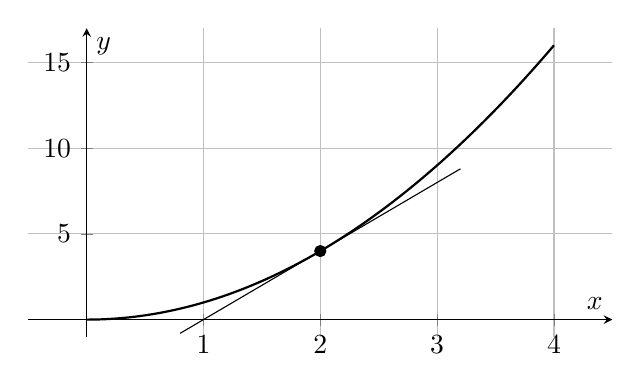
\begin{tikzpicture}
\begin{axis}[
    width=9cm,
    height=5.5cm,
    axis lines=middle,
    xmin=-0.5,xmax=4.5,
    ymin=-1,ymax=17,
    xlabel={$x$},
    ylabel={$y$},
    samples=100,
    grid=major
]
\addplot[domain=0:4,thick] {x^2};
\addplot[domain=0.8:3.2] {4*x-4};
\addplot[only marks,mark=*] coordinates {(2,4)};
\end{axis}
\end{tikzpicture}
\end{center}

%%%%%%%%%%%%%%%%%%%%%%%%%%%%%%%%%%%%%%%%%%%%%%%%%%%%%%%%%%%%
\subsection{Worked Example: Derivative from the Definition}
\label{subsec:worked-derivative-definition}
%%%%%%%%%%%%%%%%%%%%%%%%%%%%%%%%%%%%%%%%%%%%%%%%%%%%%%%%%%%%

\begin{workedexamplebox}{Derivative of \(x^2\)}

Let

\[ f(x)=x^2. \]

Find \(f'(x)\) from the definition.

\begin{tabularx}{\textwidth}{@{}>{\raggedright\arraybackslash}p{0.42\textwidth}X@{}}
Start with the definition. &
\(\displaystyle f'(x)=\lim_{h\to0}\frac{(x+h)^2-x^2}{h}\)\\
Expand. &
\(\displaystyle =\lim_{h\to0}\frac{2xh+h^2}{h}\)\\
Factor and cancel \(h\). &
\(\displaystyle =\lim_{h\to0}(2x+h)\)\\
Evaluate the limit. &
\(f'(x)=2x\)
\end{tabularx}

\begin{answerbox}
\[ \boxed{f'(x)=2x.} \]
\end{answerbox}
\end{workedexamplebox}

%%%%%%%%%%%%%%%%%%%%%%%%%%%%%%%%%%%%%%%%%%%%%%%%%%%%%%%%%%%%
\subsection{Differentiability Implies Continuity}
\label{subsec:differentiability-continuity}
%%%%%%%%%%%%%%%%%%%%%%%%%%%%%%%%%%%%%%%%%%%%%%%%%%%%%%%%%%%%

\begin{theorem}
If \(f\) is differentiable at \(a\), then \(f\) is continuous at \(a\).
\end{theorem}

The converse is false.

For example,

\[ f(x)=|x| \]

is continuous at \(0\), but its graph has a corner there, so \(f'(0)\) does
not exist.

%%%%%%%%%%%%%%%%%%%%%%%%%%%%%%%%%%%%%%%%%%%%%%%%%%%%%%%%%%%%
\subsection{Derivative Notation}
\label{subsec:derivative-notation}
%%%%%%%%%%%%%%%%%%%%%%%%%%%%%%%%%%%%%%%%%%%%%%%%%%%%%%%%%%%%

Several notations represent derivatives.

If

\[ y=f(x), \]

then the first derivative may be written

\[ f'(x),\qquad y',\qquad \frac{dy}{dx},\qquad \dv{y}{x}. \]

The expression

\[ \frac{dy}{dx} \]

is read ``the derivative of \(y\) with respect to \(x\).''

The notation suggests a ratio of infinitesimal changes and becomes especially
useful in substitution, related rates, and differential equations.

%%%%%%%%%%%%%%%%%%%%%%%%%%%%%%%%%%%%%%%%%%%%%%%%%%%%%%%%%%%%
\subsection{Higher Derivatives}
\label{subsec:higher-derivatives}
%%%%%%%%%%%%%%%%%%%%%%%%%%%%%%%%%%%%%%%%%%%%%%%%%%%%%%%%%%%%

The derivative of the derivative is the second derivative.

Common notation includes

\[ f''(x),\qquad \frac{d^2y}{dx^2}. \]

The \(n\)th derivative may be written

\[ f^{(n)}(x). \]

Higher derivatives describe higher-order change.

For position \(s(t)\),

\[ s'(t)=v(t) \]

is velocity, and

\[ s''(t)=a(t) \]

is acceleration.

%%%%%%%%%%%%%%%%%%%%%%%%%%%%%%%%%%%%%%%%%%%%%%%%%%%%%%%%%%%%
\subsection{Basic Differentiation Rules}
\label{subsec:basic-differentiation-rules}
%%%%%%%%%%%%%%%%%%%%%%%%%%%%%%%%%%%%%%%%%%%%%%%%%%%%%%%%%%%%

For a constant \(c\),

\[ \dv{}{x}c=0. \]

For \(n\) where the expression is defined appropriately,

\[ \dv{}{x}x^n=nx^{n-1}. \]

This is the \emph{Power Rule}.

If \(c\) is constant,

\[ \dv{}{x}[cf(x)]=cf'(x). \]

Also,

\[ \dv{}{x}[f(x)\pm g(x)]
=f'(x)\pm g'(x). \]

%%%%%%%%%%%%%%%%%%%%%%%%%%%%%%%%%%%%%%%%%%%%%%%%%%%%%%%%%%%%
\subsection{Product Rule}
\label{subsec:product-rule}
%%%%%%%%%%%%%%%%%%%%%%%%%%%%%%%%%%%%%%%%%%%%%%%%%%%%%%%%%%%%

\begin{theorem}[Product Rule]
If \(f\) and \(g\) are differentiable, then
\[ \dv{}{x}[f(x)g(x)]
=f'(x)g(x)+f(x)g'(x). \]
\end{theorem}

A common mistake is to write

\[ (fg)'=f'g'. \]

This is generally false.

%%%%%%%%%%%%%%%%%%%%%%%%%%%%%%%%%%%%%%%%%%%%%%%%%%%%%%%%%%%%
\subsection{Quotient Rule}
\label{subsec:quotient-rule}
%%%%%%%%%%%%%%%%%%%%%%%%%%%%%%%%%%%%%%%%%%%%%%%%%%%%%%%%%%%%

\begin{theorem}[Quotient Rule]
If \(g(x)\neq0\), then
\[ \dv{}{x}\left(\frac{f(x)}{g(x)}\right)
=
\frac{f'(x)g(x)-f(x)g'(x)}{[g(x)]^2}. \]
\end{theorem}

A useful memory form is

\[ \frac{\text{bottom}\cdot\text{derivative of top}
-\text{top}\cdot\text{derivative of bottom}}
{\text{bottom}^2}. \]

%%%%%%%%%%%%%%%%%%%%%%%%%%%%%%%%%%%%%%%%%%%%%%%%%%%%%%%%%%%%
\subsection{Chain Rule}
\label{subsec:chain-rule-calculus}
%%%%%%%%%%%%%%%%%%%%%%%%%%%%%%%%%%%%%%%%%%%%%%%%%%%%%%%%%%%%

Composition requires a special differentiation rule.

\begin{theorem}[Chain Rule]
If
\[ y=f(g(x)), \]
then
\[ \dv{y}{x}
=f'(g(x))g'(x). \]
\end{theorem}

In Leibniz notation,

\[ \dv{y}{x}=\dv{y}{u}\dv{u}{x}. \]

The chain rule differentiates the outside function and then multiplies by
the derivative of the inside function.

%%%%%%%%%%%%%%%%%%%%%%%%%%%%%%%%%%%%%%%%%%%%%%%%%%%%%%%%%%%%
\subsection{Worked Example: Chain Rule}
\label{subsec:worked-chain-rule}
%%%%%%%%%%%%%%%%%%%%%%%%%%%%%%%%%%%%%%%%%%%%%%%%%%%%%%%%%%%%

\begin{workedexamplebox}{Differentiating a Composite Function}

Differentiate

\[ f(x)=(3x^2+1)^5. \]

\begin{tabularx}{\textwidth}{@{}>{\raggedright\arraybackslash}p{0.42\textwidth}X@{}}
Identify the outer function. &
\(u^5\)\\
Differentiate the outer function. &
\(5u^4\)\\
Replace \(u\) with \(3x^2+1\). &
\(5(3x^2+1)^4\)\\
Differentiate the inside. &
\(6x\)\\
Multiply. &
\(30x(3x^2+1)^4\)
\end{tabularx}

\begin{answerbox}
\[ \boxed{f'(x)=30x(3x^2+1)^4.} \]
\end{answerbox}
\end{workedexamplebox}

%%%%%%%%%%%%%%%%%%%%%%%%%%%%%%%%%%%%%%%%%%%%%%%%%%%%%%%%%%%%
\subsection{Trigonometric Derivatives}
\label{subsec:trigonometric-derivatives}
%%%%%%%%%%%%%%%%%%%%%%%%%%%%%%%%%%%%%%%%%%%%%%%%%%%%%%%%%%%%

For radian measure,

\[ \dv{}{x}\sin x=\cos x, \]

\[ \dv{}{x}\cos x=-\sin x, \]

\[ \dv{}{x}\tan x=\sec^2x, \]

\[ \dv{}{x}\cot x=-\csc^2x, \]

\[ \dv{}{x}\sec x=\sec x\tan x, \]

and

\[ \dv{}{x}\csc x=-\csc x\cot x. \]

%%%%%%%%%%%%%%%%%%%%%%%%%%%%%%%%%%%%%%%%%%%%%%%%%%%%%%%%%%%%
\subsection{Exponential Derivatives}
\label{subsec:exponential-derivatives}
%%%%%%%%%%%%%%%%%%%%%%%%%%%%%%%%%%%%%%%%%%%%%%%%%%%%%%%%%%%%

The natural exponential function satisfies

\[ \boxed{\dv{}{x}e^x=e^x.} \]

More generally,

\[ \dv{}{x}a^x=a^x\ln a. \]

For a differentiable function \(u(x)\),

\[ \dv{}{x}e^{u(x)}=e^{u(x)}u'(x). \]

%%%%%%%%%%%%%%%%%%%%%%%%%%%%%%%%%%%%%%%%%%%%%%%%%%%%%%%%%%%%
\subsection{Logarithmic Derivatives}
\label{subsec:logarithmic-derivatives}
%%%%%%%%%%%%%%%%%%%%%%%%%%%%%%%%%%%%%%%%%%%%%%%%%%%%%%%%%%%%

For \(x>0\),

\[ \boxed{\dv{}{x}\ln x=\frac1x.} \]

More generally,

\[ \dv{}{x}\ln|x|=\frac1x,\qquad x\neq0. \]

For base \(a\),

\[ \dv{}{x}\log_a x=\frac{1}{x\ln a}. \]

By the chain rule,

\[ \dv{}{x}\ln|u(x)|=\frac{u'(x)}{u(x)} \]

whenever \(u(x)\neq0\).

%%%%%%%%%%%%%%%%%%%%%%%%%%%%%%%%%%%%%%%%%%%%%%%%%%%%%%%%%%%%
\subsection{Inverse Trigonometric Derivatives}
\label{subsec:inverse-trigonometric-derivatives}
%%%%%%%%%%%%%%%%%%%%%%%%%%%%%%%%%%%%%%%%%%%%%%%%%%%%%%%%%%%%

Important formulas include

\[ \dv{}{x}\arcsin x=\frac1{\sqrt{1-x^2}}, \]

\[ \dv{}{x}\arccos x=-\frac1{\sqrt{1-x^2}}, \]

and

\[ \dv{}{x}\arctan x=\frac1{1+x^2}. \]

Additional formulas include

\[ \dv{}{x}\operatorname{arccot}x=-\frac1{1+x^2}, \]

\[ \dv{}{x}\operatorname{arcsec}x
=\frac1{|x|\sqrt{x^2-1}}, \]

and

\[ \dv{}{x}\operatorname{arccsc}x
=-\frac1{|x|\sqrt{x^2-1}}. \]

%%%%%%%%%%%%%%%%%%%%%%%%%%%%%%%%%%%%%%%%%%%%%%%%%%%%%%%%%%%%
\subsection{Implicit Differentiation}
\label{subsec:implicit-differentiation}
%%%%%%%%%%%%%%%%%%%%%%%%%%%%%%%%%%%%%%%%%%%%%%%%%%%%%%%%%%%%

Not every relationship is naturally solved for \(y\).

Suppose

\[ x^2+y^2=25. \]

Differentiate both sides with respect to \(x\):

\[ 2x+2y\dv{y}{x}=0. \]

Solve for the derivative:

\[ \boxed{\dv{y}{x}=-\frac{x}{y}.} \]

The chain rule is used whenever differentiating an expression involving
\(y(x)\).

%%%%%%%%%%%%%%%%%%%%%%%%%%%%%%%%%%%%%%%%%%%%%%%%%%%%%%%%%%%%
\subsection{Worked Example: Implicit Differentiation}
\label{subsec:worked-implicit}
%%%%%%%%%%%%%%%%%%%%%%%%%%%%%%%%%%%%%%%%%%%%%%%%%%%%%%%%%%%%

\begin{workedexamplebox}{Implicit Derivative}

Find \(dy/dx\) if

\[ x^3+y^3=6xy. \]

\begin{tabularx}{\textwidth}{@{}>{\raggedright\arraybackslash}p{0.42\textwidth}X@{}}
Differentiate both sides. &
\(3x^2+3y^2y'=6(y+xy')\)\\
Collect terms involving \(y'\). &
\(3y^2y'-6xy'=6y-3x^2\)\\
Factor. &
\(y'(3y^2-6x)=6y-3x^2\)\\
Solve for \(y'\). &
\(\displaystyle y'=\frac{6y-3x^2}{3y^2-6x}\)
\end{tabularx}

\begin{answerbox}
\[ \boxed{\dv{y}{x}=\frac{2y-x^2}{y^2-2x}.} \]
\end{answerbox}
\end{workedexamplebox}

%%%%%%%%%%%%%%%%%%%%%%%%%%%%%%%%%%%%%%%%%%%%%%%%%%%%%%%%%%%%
\subsection{Logarithmic Differentiation}
\label{subsec:logarithmic-differentiation}
%%%%%%%%%%%%%%%%%%%%%%%%%%%%%%%%%%%%%%%%%%%%%%%%%%%%%%%%%%%%

Products, quotients, powers, or variable exponents can sometimes be
simplified by first taking logarithms.

Suppose

\[ y=x^x,\qquad x>0. \]

Take natural logarithms:

\[ \ln y=x\ln x. \]

Differentiate:

\[ \frac{y'}{y}=\ln x+1. \]

Thus

\[ \boxed{y'=x^x(\ln x+1).} \]

%%%%%%%%%%%%%%%%%%%%%%%%%%%%%%%%%%%%%%%%%%%%%%%%%%%%%%%%%%%%
\subsection{Tangent and Normal Lines}
\label{subsec:tangent-normal-lines}
%%%%%%%%%%%%%%%%%%%%%%%%%%%%%%%%%%%%%%%%%%%%%%%%%%%%%%%%%%%%

At \(x=a\), the tangent slope is

\[ m_{\mathrm{tan}}=f'(a). \]

Therefore the tangent line is

\[ y-f(a)=f'(a)(x-a). \]

If \(f'(a)\neq0\), the normal line is perpendicular to the tangent and has
slope

\[ m_{\mathrm{normal}}=-\frac1{f'(a)}. \]

%%%%%%%%%%%%%%%%%%%%%%%%%%%%%%%%%%%%%%%%%%%%%%%%%%%%%%%%%%%%
\subsection{Linear Approximation}
\label{subsec:linear-approximation}
%%%%%%%%%%%%%%%%%%%%%%%%%%%%%%%%%%%%%%%%%%%%%%%%%%%%%%%%%%%%

Near \(x=a\), a differentiable function behaves approximately like its
tangent line.

The linearization is

\[ L(x)=f(a)+f'(a)(x-a). \]

For \(x\) near \(a\),

\[ f(x)\approx L(x). \]

This is the first local approximation produced by calculus.

%%%%%%%%%%%%%%%%%%%%%%%%%%%%%%%%%%%%%%%%%%%%%%%%%%%%%%%%%%%%
\subsection{Differentials}
\label{subsec:differentials}
%%%%%%%%%%%%%%%%%%%%%%%%%%%%%%%%%%%%%%%%%%%%%%%%%%%%%%%%%%%%

If

\[ y=f(x), \]

then the differential \(dy\) is defined by

\[ dy=f'(x)\,dx. \]

For a small change \(\Delta x\),

\[ \Delta y\approx dy. \]

Differentials provide a useful language for approximation, error analysis,
substitution, and differential equations.

%%%%%%%%%%%%%%%%%%%%%%%%%%%%%%%%%%%%%%%%%%%%%%%%%%%%%%%%%%%%
\subsection{Related Rates}
\label{subsec:related-rates}
%%%%%%%%%%%%%%%%%%%%%%%%%%%%%%%%%%%%%%%%%%%%%%%%%%%%%%%%%%%%

When several quantities depend on time, their rates of change may be related
through an equation.

The standard method is:

\begin{enumerate}
    \item identify changing quantities;
    \item write an equation relating them;
    \item differentiate with respect to time;
    \item substitute known values;
    \item solve for the desired rate.
\end{enumerate}

%%%%%%%%%%%%%%%%%%%%%%%%%%%%%%%%%%%%%%%%%%%%%%%%%%%%%%%%%%%%
\subsection{Worked Example: Related Rates}
\label{subsec:worked-related-rates}
%%%%%%%%%%%%%%%%%%%%%%%%%%%%%%%%%%%%%%%%%%%%%%%%%%%%%%%%%%%%

\begin{workedexamplebox}{Expanding Circle}

A circle's radius increases at

\[ \dv{r}{t}=2\text{ cm/s}. \]

Find the rate of change of its area when \(r=5\) cm.

\begin{tabularx}{\textwidth}{@{}>{\raggedright\arraybackslash}p{0.42\textwidth}X@{}}
Start with the area formula. &
\(A=\pi r^2\)\\
Differentiate with respect to \(t\). &
\(\displaystyle \dv{A}{t}=2\pi r\dv{r}{t}\)\\
Substitute \(r=5\) and \(dr/dt=2\). &
\(\displaystyle \dv{A}{t}=2\pi(5)(2)\)\\
Simplify. &
\(\displaystyle \dv{A}{t}=20\pi\)
\end{tabularx}

\begin{answerbox}
\[ \boxed{\dv{A}{t}=20\pi\text{ cm}^2/\text{s}.} \]
\end{answerbox}
\end{workedexamplebox}

%%%%%%%%%%%%%%%%%%%%%%%%%%%%%%%%%%%%%%%%%%%%%%%%%%%%%%%%%%%%
\subsection{Critical Numbers}
\label{subsec:critical-numbers}
%%%%%%%%%%%%%%%%%%%%%%%%%%%%%%%%%%%%%%%%%%%%%%%%%%%%%%%%%%%%

\begin{definitionbox}{Critical Number}
A number \(c\) in the domain of \(f\) is a \emph{critical number} if
\[ f'(c)=0 \]
or \(f'(c)\) does not exist.
\end{definitionbox}

Local extrema can occur at critical numbers.

They may also occur at endpoints of restricted domains.

%%%%%%%%%%%%%%%%%%%%%%%%%%%%%%%%%%%%%%%%%%%%%%%%%%%%%%%%%%%%
\subsection{Fermat's Theorem}
\label{subsec:fermats-theorem-calculus}
%%%%%%%%%%%%%%%%%%%%%%%%%%%%%%%%%%%%%%%%%%%%%%%%%%%%%%%%%%%%

\begin{theorem}[Fermat's Theorem]
If \(f\) has a local maximum or minimum at an interior point \(c\) and is
differentiable at \(c\), then
\[ f'(c)=0. \]
\end{theorem}

The converse is not true.

A point satisfying \(f'(c)=0\) need not be an extremum.

%%%%%%%%%%%%%%%%%%%%%%%%%%%%%%%%%%%%%%%%%%%%%%%%%%%%%%%%%%%%
\subsection{Rolle's Theorem}
\label{subsec:rolles-theorem}
%%%%%%%%%%%%%%%%%%%%%%%%%%%%%%%%%%%%%%%%%%%%%%%%%%%%%%%%%%%%

\begin{theorem}[Rolle's Theorem]
Suppose:
\begin{enumerate}
    \item \(f\) is continuous on \([a,b]\);
    \item \(f\) is differentiable on \((a,b)\);
    \item \(f(a)=f(b)\).
\end{enumerate}
Then there exists \(c\in(a,b)\) such that
\[ f'(c)=0. \]
\end{theorem}

Geometrically, some tangent line must be horizontal.

%%%%%%%%%%%%%%%%%%%%%%%%%%%%%%%%%%%%%%%%%%%%%%%%%%%%%%%%%%%%
\subsection{Mean Value Theorem}
\label{subsec:mean-value-theorem}
%%%%%%%%%%%%%%%%%%%%%%%%%%%%%%%%%%%%%%%%%%%%%%%%%%%%%%%%%%%%

\begin{theorem}[Mean Value Theorem]
Suppose \(f\) is continuous on \([a,b]\) and differentiable on \((a,b)\).
Then there exists \(c\in(a,b)\) such that
\[ f'(c)=\frac{f(b)-f(a)}{b-a}. \]
\end{theorem}

Thus at some point, the instantaneous rate of change equals the average rate
of change over the interval.

%%%%%%%%%%%%%%%%%%%%%%%%%%%%%%%%%%%%%%%%%%%%%%%%%%%%%%%%%%%%
\subsection{Increasing and Decreasing from the Derivative}
\label{subsec:derivative-monotonicity}
%%%%%%%%%%%%%%%%%%%%%%%%%%%%%%%%%%%%%%%%%%%%%%%%%%%%%%%%%%%%

If

\[ f'(x)>0 \]

throughout an interval, then \(f\) is increasing there.

If

\[ f'(x)<0, \]

then \(f\) is decreasing.

This gives a systematic way to analyze function behavior.

%%%%%%%%%%%%%%%%%%%%%%%%%%%%%%%%%%%%%%%%%%%%%%%%%%%%%%%%%%%%
\subsection{First Derivative Test}
\label{subsec:first-derivative-test}
%%%%%%%%%%%%%%%%%%%%%%%%%%%%%%%%%%%%%%%%%%%%%%%%%%%%%%%%%%%%

Suppose \(c\) is a critical number.

If \(f'\) changes from positive to negative at \(c\), then \(f\) has a local
maximum at \(c\).

If \(f'\) changes from negative to positive, then \(f\) has a local minimum.

If the sign does not change, there is no local extremum detected by this
test.

%%%%%%%%%%%%%%%%%%%%%%%%%%%%%%%%%%%%%%%%%%%%%%%%%%%%%%%%%%%%
\subsection{Concavity}
\label{subsec:concavity}
%%%%%%%%%%%%%%%%%%%%%%%%%%%%%%%%%%%%%%%%%%%%%%%%%%%%%%%%%%%%

The second derivative describes how slopes change.

If

\[ f''(x)>0, \]

the graph is concave upward.

If

\[ f''(x)<0, \]

the graph is concave downward.

Geometrically, concavity describes the direction in which the graph bends.

%%%%%%%%%%%%%%%%%%%%%%%%%%%%%%%%%%%%%%%%%%%%%%%%%%%%%%%%%%%%
\subsection{Inflection Points}
\label{subsec:inflection-points}
%%%%%%%%%%%%%%%%%%%%%%%%%%%%%%%%%%%%%%%%%%%%%%%%%%%%%%%%%%%%

A point of inflection occurs where the concavity changes.

Candidates often occur where

\[ f''(x)=0 \]

or where \(f''\) fails to exist.

However, simply solving \(f''(x)=0\) is not sufficient.

The sign of \(f''\) must actually change.

%%%%%%%%%%%%%%%%%%%%%%%%%%%%%%%%%%%%%%%%%%%%%%%%%%%%%%%%%%%%
\subsection{Second Derivative Test}
\label{subsec:second-derivative-test}
%%%%%%%%%%%%%%%%%%%%%%%%%%%%%%%%%%%%%%%%%%%%%%%%%%%%%%%%%%%%

Suppose

\[ f'(c)=0. \]

If

\[ f''(c)>0, \]

then \(f\) has a local minimum at \(c\).

If

\[ f''(c)<0, \]

then \(f\) has a local maximum at \(c\).

If

\[ f''(c)=0, \]

the test is inconclusive.

%%%%%%%%%%%%%%%%%%%%%%%%%%%%%%%%%%%%%%%%%%%%%%%%%%%%%%%%%%%%
\subsection{Curve Analysis}
\label{subsec:curve-analysis-calculus}
%%%%%%%%%%%%%%%%%%%%%%%%%%%%%%%%%%%%%%%%%%%%%%%%%%%%%%%%%%%%

A systematic graph analysis may include:

\begin{enumerate}
    \item domain;
    \item intercepts;
    \item symmetry;
    \item asymptotes;
    \item critical numbers;
    \item increasing and decreasing intervals;
    \item local and absolute extrema;
    \item concavity;
    \item inflection points;
    \item end behavior.
\end{enumerate}

Calculus combines these pieces to produce a detailed understanding of the
graph.

%%%%%%%%%%%%%%%%%%%%%%%%%%%%%%%%%%%%%%%%%%%%%%%%%%%%%%%%%%%%
\subsection{Optimization}
\label{subsec:optimization-calculus}
%%%%%%%%%%%%%%%%%%%%%%%%%%%%%%%%%%%%%%%%%%%%%%%%%%%%%%%%%%%%

Optimization problems ask for maximum or minimum values subject to
constraints.

The standard process is:

\begin{enumerate}
    \item identify the objective quantity;
    \item write the objective as a function;
    \item use constraints to reduce to one variable;
    \item determine the relevant domain;
    \item find critical numbers;
    \item test critical numbers and endpoints;
    \item interpret the result.
\end{enumerate}

%%%%%%%%%%%%%%%%%%%%%%%%%%%%%%%%%%%%%%%%%%%%%%%%%%%%%%%%%%%%
\subsection{Worked Example: Optimization}
\label{subsec:worked-optimization}
%%%%%%%%%%%%%%%%%%%%%%%%%%%%%%%%%%%%%%%%%%%%%%%%%%%%%%%%%%%%

\begin{workedexamplebox}{Maximum Area with Fixed Perimeter}

A rectangle has perimeter \(40\). Find the dimensions giving maximum area.

\begin{tabularx}{\textwidth}{@{}>{\raggedright\arraybackslash}p{0.42\textwidth}X@{}}
Let the sides be \(x\) and \(y\). &
\(2x+2y=40\)\\
Solve the constraint. &
\(y=20-x\)\\
Write area as one variable. &
\(A(x)=x(20-x)=20x-x^2\)\\
Differentiate. &
\(A'(x)=20-2x\)\\
Find the critical point. &
\(20-2x=0\Rightarrow x=10\)\\
Find the other side. &
\(y=10\)
\end{tabularx}

\begin{answerbox}
\[ \boxed{10\times10\text{ gives the maximum area.}} \]
\end{answerbox}
\end{workedexamplebox}

%%%%%%%%%%%%%%%%%%%%%%%%%%%%%%%%%%%%%%%%%%%%%%%%%%%%%%%%%%%%
\subsection{L'Hospital's Rule}
\label{subsec:lhospital-rule}
%%%%%%%%%%%%%%%%%%%%%%%%%%%%%%%%%%%%%%%%%%%%%%%%%%%%%%%%%%%%

Some indeterminate limits can be evaluated using derivatives.

\begin{theorem}[L'Hospital's Rule]
Under appropriate hypotheses, if
\[ \lim_{x\to a}\frac{f(x)}{g(x)} \]
has the indeterminate form \(0/0\) or \(\infty/\infty\), then
\[ \lim_{x\to a}\frac{f(x)}{g(x)}
=
\lim_{x\to a}\frac{f'(x)}{g'(x)}, \]
provided the latter limit exists or has the appropriate infinite behavior.
\end{theorem}

This rule applies to quotients of functions, not arbitrary expressions.

%%%%%%%%%%%%%%%%%%%%%%%%%%%%%%%%%%%%%%%%%%%%%%%%%%%%%%%%%%%%
\subsection{Antiderivatives}
\label{subsec:antiderivatives}
%%%%%%%%%%%%%%%%%%%%%%%%%%%%%%%%%%%%%%%%%%%%%%%%%%%%%%%%%%%%

Differentiation asks:

\begin{quote}
Given \(F\), what is \(F'\)?
\end{quote}

Antidifferentiation reverses this question.

\begin{definitionbox}{Antiderivative}
A function \(F\) is an \emph{antiderivative} of \(f\) on an interval if
\[ F'(x)=f(x) \]
throughout that interval.
\end{definitionbox}

For example, since

\[ \dv{}{x}x^3=3x^2, \]

an antiderivative of \(3x^2\) is

\[ x^3. \]

%%%%%%%%%%%%%%%%%%%%%%%%%%%%%%%%%%%%%%%%%%%%%%%%%%%%%%%%%%%%
\subsection{Indefinite Integrals}
\label{subsec:indefinite-integrals}
%%%%%%%%%%%%%%%%%%%%%%%%%%%%%%%%%%%%%%%%%%%%%%%%%%%%%%%%%%%%

The family of all antiderivatives of \(f\) is written

\[ \int f(x)\,dx=F(x)+C. \]

The symbol

\[ \int \]

is called the \emph{integral sign} and is read ``integral.''

The expression

\[ dx \]

indicates the variable of integration and is read ``with respect to \(x\).''

The constant

\[ C \]

is called the constant of integration.

%%%%%%%%%%%%%%%%%%%%%%%%%%%%%%%%%%%%%%%%%%%%%%%%%%%%%%%%%%%%
\subsection{Basic Antiderivative Rules}
\label{subsec:basic-antiderivative-rules}
%%%%%%%%%%%%%%%%%%%%%%%%%%%%%%%%%%%%%%%%%%%%%%%%%%%%%%%%%%%%

For \(n\neq-1\),

\[ \int x^n\,dx=\frac{x^{n+1}}{n+1}+C. \]

Also,

\[ \int \frac1x\,dx=\ln|x|+C. \]

For constants \(a,b\),

\[ \int [af(x)+bg(x)]\,dx
=a\int f(x)\,dx+b\int g(x)\,dx. \]

%%%%%%%%%%%%%%%%%%%%%%%%%%%%%%%%%%%%%%%%%%%%%%%%%%%%%%%%%%%%
\subsection{Basic Trigonometric Antiderivatives}
\label{subsec:trig-antiderivatives}
%%%%%%%%%%%%%%%%%%%%%%%%%%%%%%%%%%%%%%%%%%%%%%%%%%%%%%%%%%%%

Important formulas include

\[ \int\cos x\,dx=\sin x+C, \]

\[ \int\sin x\,dx=-\cos x+C, \]

\[ \int\sec^2x\,dx=\tan x+C, \]

\[ \int\csc^2x\,dx=-\cot x+C, \]

\[ \int\sec x\tan x\,dx=\sec x+C, \]

and

\[ \int\csc x\cot x\,dx=-\csc x+C. \]

%%%%%%%%%%%%%%%%%%%%%%%%%%%%%%%%%%%%%%%%%%%%%%%%%%%%%%%%%%%%
\subsection{Exponential Antiderivatives}
\label{subsec:exponential-antiderivatives}
%%%%%%%%%%%%%%%%%%%%%%%%%%%%%%%%%%%%%%%%%%%%%%%%%%%%%%%%%%%%

Because

\[ \dv{}{x}e^x=e^x, \]

we have

\[ \int e^x\,dx=e^x+C. \]

For \(a>0\), \(a\neq1\),

\[ \int a^x\,dx=\frac{a^x}{\ln a}+C. \]

%%%%%%%%%%%%%%%%%%%%%%%%%%%%%%%%%%%%%%%%%%%%%%%%%%%%%%%%%%%%
\subsection{Initial Value Problems}
\label{subsec:initial-value-problems-antiderivatives}
%%%%%%%%%%%%%%%%%%%%%%%%%%%%%%%%%%%%%%%%%%%%%%%%%%%%%%%%%%%%

An antiderivative family contains an arbitrary constant.

An initial condition selects one particular member.

For example, suppose

\[ F'(x)=2x,\qquad F(1)=5. \]

Integrating,

\[ F(x)=x^2+C. \]

Using \(F(1)=5\),

\[ 1+C=5, \]

so

\[ C=4. \]

Thus

\[ \boxed{F(x)=x^2+4.} \]

%%%%%%%%%%%%%%%%%%%%%%%%%%%%%%%%%%%%%%%%%%%%%%%%%%%%%%%%%%%%
\subsection{Area and Accumulation}
\label{subsec:area-accumulation}
%%%%%%%%%%%%%%%%%%%%%%%%%%%%%%%%%%%%%%%%%%%%%%%%%%%%%%%%%%%%

The second major problem of calculus concerns accumulated quantities.

For a nonnegative function, one may ask for the area under the curve from
\(x=a\) to \(x=b\).

The key idea is to approximate the region using rectangles and then let the
rectangles become arbitrarily narrow.

This limiting process produces the definite integral.

%%%%%%%%%%%%%%%%%%%%%%%%%%%%%%%%%%%%%%%%%%%%%%%%%%%%%%%%%%%%
\subsection{Riemann Sums}
\label{subsec:riemann-sums}
%%%%%%%%%%%%%%%%%%%%%%%%%%%%%%%%%%%%%%%%%%%%%%%%%%%%%%%%%%%%

Divide

\[ [a,b] \]

into \(n\) subintervals.

For equal widths,

\[ \Delta x=\frac{b-a}{n}. \]

Choose a sample point \(x_i^*\) from each subinterval.

The corresponding Riemann sum is

\[ \sum_{i=1}^{n}f(x_i^*)\Delta x. \]

The uppercase Greek letter

\[ \Sigma \]

is sigma, pronounced ``SIG-muh.''

The symbol

\[ \sum \]

is the summation symbol and is read ``the sum.''

%%%%%%%%%%%%%%%%%%%%%%%%%%%%%%%%%%%%%%%%%%%%%%%%%%%%%%%%%%%%
\subsection{Definite Integral}
\label{subsec:definite-integral}
%%%%%%%%%%%%%%%%%%%%%%%%%%%%%%%%%%%%%%%%%%%%%%%%%%%%%%%%%%%%

\begin{definitionbox}{Definite Integral}
If the limit exists, the definite integral of \(f\) from \(a\) to \(b\) is
\[ \int_a^b f(x)\,dx
=
\lim_{n\to\infty}
\sum_{i=1}^{n}f(x_i^*)\Delta x. \]
\end{definitionbox}

The notation is read:

``the integral from \(a\) to \(b\) of \(f(x)\) with respect to \(x\).''

The numbers \(a\) and \(b\) are called the limits of integration.

%%%%%%%%%%%%%%%%%%%%%%%%%%%%%%%%%%%%%%%%%%%%%%%%%%%%%%%%%%%%
\subsection{Signed Area}
\label{subsec:signed-area}
%%%%%%%%%%%%%%%%%%%%%%%%%%%%%%%%%%%%%%%%%%%%%%%%%%%%%%%%%%%%

The definite integral measures signed accumulation.

Regions above the \(x\)-axis contribute positively.

Regions below the \(x\)-axis contribute negatively.

Therefore,

\[ \int_a^b f(x)\,dx \]

is not always the ordinary geometric area.

If geometric area is desired, one may need to integrate

\[ |f(x)| \]

or split the interval at zeros of the function.

%%%%%%%%%%%%%%%%%%%%%%%%%%%%%%%%%%%%%%%%%%%%%%%%%%%%%%%%%%%%
\subsection{Properties of Definite Integrals}
\label{subsec:definite-integral-properties}
%%%%%%%%%%%%%%%%%%%%%%%%%%%%%%%%%%%%%%%%%%%%%%%%%%%%%%%%%%%%

Important properties include

\[ \int_a^a f(x)\,dx=0, \]

\[ \int_a^b f(x)\,dx=-\int_b^a f(x)\,dx, \]

and for \(a<c<b\),

\[ \int_a^b f(x)\,dx
=
\int_a^c f(x)\,dx
+
\int_c^b f(x)\,dx. \]

Linearity gives

\[ \int_a^b[cf(x)+dg(x)]\,dx
=
c\int_a^b f(x)\,dx
+
d\int_a^b g(x)\,dx. \]

%%%%%%%%%%%%%%%%%%%%%%%%%%%%%%%%%%%%%%%%%%%%%%%%%%%%%%%%%%%%
\subsection{Fundamental Theorem of Calculus}
\label{subsec:fundamental-theorem-calculus}
%%%%%%%%%%%%%%%%%%%%%%%%%%%%%%%%%%%%%%%%%%%%%%%%%%%%%%%%%%%%

The Fundamental Theorem of Calculus connects differentiation and
integration.

\begin{theorem}[Fundamental Theorem of Calculus, Part I]
If \(f\) is continuous on an interval and
\[ F(x)=\int_a^x f(t)\,dt, \]
then
\[ F'(x)=f(x). \]
\end{theorem}

Thus accumulating a function and then differentiating recovers the original
function.

%%%%%%%%%%%%%%%%%%%%%%%%%%%%%%%%%%%%%%%%%%%%%%%%%%%%%%%%%%%%
\subsection{Fundamental Theorem of Calculus Part II}
\label{subsec:ftc-part-two}
%%%%%%%%%%%%%%%%%%%%%%%%%%%%%%%%%%%%%%%%%%%%%%%%%%%%%%%%%%%%

\begin{theorem}[Fundamental Theorem of Calculus, Part II]
If \(F'(x)=f(x)\) on \([a,b]\), then
\[ \int_a^b f(x)\,dx=F(b)-F(a). \]
\end{theorem}

The notation

\[ F(b)-F(a) \]

is sometimes written

\[ \evalat{F(x)}{a}{b}. \]

This is read ``\(F(x)\) evaluated from \(a\) to \(b\).''

%%%%%%%%%%%%%%%%%%%%%%%%%%%%%%%%%%%%%%%%%%%%%%%%%%%%%%%%%%%%
\subsection{Worked Example: Definite Integral}
\label{subsec:worked-definite-integral}
%%%%%%%%%%%%%%%%%%%%%%%%%%%%%%%%%%%%%%%%%%%%%%%%%%%%%%%%%%%%

\begin{workedexamplebox}{Using the Fundamental Theorem}

Evaluate

\[ \int_0^2(3x^2+1)\,dx. \]

\begin{tabularx}{\textwidth}{@{}>{\raggedright\arraybackslash}p{0.42\textwidth}X@{}}
Find an antiderivative. &
\(F(x)=x^3+x\)\\
Apply the Fundamental Theorem. &
\(\displaystyle F(2)-F(0)\)\\
Evaluate. &
\((8+2)-0=10\)
\end{tabularx}

\begin{answerbox}
\[ \boxed{\int_0^2(3x^2+1)\,dx=10.} \]
\end{answerbox}
\end{workedexamplebox}

%%%%%%%%%%%%%%%%%%%%%%%%%%%%%%%%%%%%%%%%%%%%%%%%%%%%%%%%%%%%
\subsection{Accumulation Functions}
\label{subsec:accumulation-functions}
%%%%%%%%%%%%%%%%%%%%%%%%%%%%%%%%%%%%%%%%%%%%%%%%%%%%%%%%%%%%

A function of the form

\[ A(x)=\int_a^x f(t)\,dt \]

is called an accumulation function.

It measures the net accumulation of \(f\) from \(a\) to \(x\).

By the Fundamental Theorem,

\[ A'(x)=f(x). \]

Thus the original function gives the instantaneous rate of accumulation.

%%%%%%%%%%%%%%%%%%%%%%%%%%%%%%%%%%%%%%%%%%%%%%%%%%%%%%%%%%%%
\subsection{Substitution}
\label{subsec:substitution}
%%%%%%%%%%%%%%%%%%%%%%%%%%%%%%%%%%%%%%%%%%%%%%%%%%%%%%%%%%%%

Substitution reverses the chain rule.

Suppose an integral contains

\[ f(g(x))g'(x). \]

Set

\[ u=g(x). \]

Then

\[ du=g'(x)\,dx. \]

The integral becomes

\[ \int f(u)\,du. \]

This method is called \emph{\(u\)-substitution}.

%%%%%%%%%%%%%%%%%%%%%%%%%%%%%%%%%%%%%%%%%%%%%%%%%%%%%%%%%%%%
\subsection{Worked Example: Substitution}
\label{subsec:worked-substitution}
%%%%%%%%%%%%%%%%%%%%%%%%%%%%%%%%%%%%%%%%%%%%%%%%%%%%%%%%%%%%

\begin{workedexamplebox}{Using \(u\)-Substitution}

Evaluate

\[ \int 2x(x^2+1)^4\,dx. \]

\begin{tabularx}{\textwidth}{@{}>{\raggedright\arraybackslash}p{0.42\textwidth}X@{}}
Choose the inner expression. &
\(u=x^2+1\)\\
Differentiate. &
\(du=2x\,dx\)\\
Rewrite the integral. &
\(\displaystyle \int u^4\,du\)\\
Integrate. &
\(\displaystyle \frac{u^5}{5}+C\)\\
Substitute back. &
\(\displaystyle \frac{(x^2+1)^5}{5}+C\)
\end{tabularx}

\begin{answerbox}
\[ \boxed{\int 2x(x^2+1)^4\,dx
=\frac{(x^2+1)^5}{5}+C.} \]
\end{answerbox}
\end{workedexamplebox}

%%%%%%%%%%%%%%%%%%%%%%%%%%%%%%%%%%%%%%%%%%%%%%%%%%%%%%%%%%%%
\subsection{Substitution in Definite Integrals}
\label{subsec:definite-substitution}
%%%%%%%%%%%%%%%%%%%%%%%%%%%%%%%%%%%%%%%%%%%%%%%%%%%%%%%%%%%%

For definite integrals, one may transform the bounds.

If

\[ u=g(x), \]

then when

\[ x=a,\qquad u=g(a), \]

and when

\[ x=b,\qquad u=g(b). \]

Thus

\[ \int_a^b f(g(x))g'(x)\,dx
=
\int_{g(a)}^{g(b)}f(u)\,du. \]

Once the bounds are changed, there is no need to substitute back to \(x\).

%%%%%%%%%%%%%%%%%%%%%%%%%%%%%%%%%%%%%%%%%%%%%%%%%%%%%%%%%%%%
\subsection{Area Between Curves}
\label{subsec:area-between-curves}
%%%%%%%%%%%%%%%%%%%%%%%%%%%%%%%%%%%%%%%%%%%%%%%%%%%%%%%%%%%%

If

\[ f(x)\geq g(x) \]

on \([a,b]\), then the area between the curves is

\[ A=\int_a^b[f(x)-g(x)]\,dx. \]

A useful memory rule is

\[ \boxed{\text{area}=\int(\text{top}-\text{bottom})\,dx.} \]

If integrating with respect to \(y\), use

\[ \boxed{\text{area}=\int(\text{right}-\text{left})\,dy.} \]

%%%%%%%%%%%%%%%%%%%%%%%%%%%%%%%%%%%%%%%%%%%%%%%%%%%%%%%%%%%%
\subsection{Average Value of a Function}
\label{subsec:average-value}
%%%%%%%%%%%%%%%%%%%%%%%%%%%%%%%%%%%%%%%%%%%%%%%%%%%%%%%%%%%%

The average value of \(f\) on \([a,b]\) is

\[ f_{\mathrm{avg}}
=
\frac1{b-a}\int_a^b f(x)\,dx. \]

This generalizes the ordinary arithmetic average to continuously varying
quantities.

%%%%%%%%%%%%%%%%%%%%%%%%%%%%%%%%%%%%%%%%%%%%%%%%%%%%%%%%%%%%
\subsection{Mean Value Theorem for Integrals}
\label{subsec:mean-value-integrals}
%%%%%%%%%%%%%%%%%%%%%%%%%%%%%%%%%%%%%%%%%%%%%%%%%%%%%%%%%%%%

\begin{theorem}[Mean Value Theorem for Integrals]
If \(f\) is continuous on \([a,b]\), then there exists \(c\in[a,b]\) such
that
\[ f(c)=\frac1{b-a}\int_a^b f(x)\,dx. \]
\end{theorem}

Thus at some point the function equals its average value.

%%%%%%%%%%%%%%%%%%%%%%%%%%%%%%%%%%%%%%%%%%%%%%%%%%%%%%%%%%%%
\subsection{Position, Velocity, and Acceleration}
\label{subsec:motion-calculus}
%%%%%%%%%%%%%%%%%%%%%%%%%%%%%%%%%%%%%%%%%%%%%%%%%%%%%%%%%%%%

If \(s(t)\) is position, then

\[ v(t)=s'(t) \]

is velocity, and

\[ a(t)=v'(t)=s''(t) \]

is acceleration.

Conversely,

\[ v(t)=v(t_0)+\int_{t_0}^t a(u)\,du, \]

and

\[ s(t)=s(t_0)+\int_{t_0}^t v(u)\,du. \]

Thus differentiation gives rates, while integration reconstructs quantities
from their rates.

%%%%%%%%%%%%%%%%%%%%%%%%%%%%%%%%%%%%%%%%%%%%%%%%%%%%%%%%%%%%
\subsection{Displacement and Distance}
\label{subsec:displacement-distance}
%%%%%%%%%%%%%%%%%%%%%%%%%%%%%%%%%%%%%%%%%%%%%%%%%%%%%%%%%%%%

If \(v(t)\) is velocity, displacement from \(t=a\) to \(t=b\) is

\[ \int_a^b v(t)\,dt. \]

Total distance traveled is

\[ \int_a^b|v(t)|\,dt. \]

These are generally different because displacement is signed while distance
is nonnegative.

%%%%%%%%%%%%%%%%%%%%%%%%%%%%%%%%%%%%%%%%%%%%%%%%%%%%%%%%%%%%
\subsection{Volumes by Slicing}
\label{subsec:volumes-slicing}
%%%%%%%%%%%%%%%%%%%%%%%%%%%%%%%%%%%%%%%%%%%%%%%%%%%%%%%%%%%%

Suppose a solid has cross-sectional area \(A(x)\).

Its volume from \(x=a\) to \(x=b\) is

\[ V=\int_a^b A(x)\,dx. \]

This formula is the general foundation for disk, washer, and other slicing
methods.

%%%%%%%%%%%%%%%%%%%%%%%%%%%%%%%%%%%%%%%%%%%%%%%%%%%%%%%%%%%%
\subsection{Disk Method}
\label{subsec:disk-method}
%%%%%%%%%%%%%%%%%%%%%%%%%%%%%%%%%%%%%%%%%%%%%%%%%%%%%%%%%%%%

If rotating

\[ y=f(x)\geq0 \]

around the \(x\)-axis, each cross section is a disk of radius \(f(x)\).

Thus

\[ A(x)=\pi[f(x)]^2, \]

and

\[ \boxed{V=\pi\int_a^b[f(x)]^2\,dx.} \]

%%%%%%%%%%%%%%%%%%%%%%%%%%%%%%%%%%%%%%%%%%%%%%%%%%%%%%%%%%%%
\subsection{Washer Method}
\label{subsec:washer-method}
%%%%%%%%%%%%%%%%%%%%%%%%%%%%%%%%%%%%%%%%%%%%%%%%%%%%%%%%%%%%

If a cross section has outer radius \(R(x)\) and inner radius \(r(x)\), then

\[ A(x)=\pi[R(x)]^2-\pi[r(x)]^2. \]

Therefore,

\[ \boxed{
V=\pi\int_a^b
\left(R(x)^2-r(x)^2\right)\,dx.
} \]

%%%%%%%%%%%%%%%%%%%%%%%%%%%%%%%%%%%%%%%%%%%%%%%%%%%%%%%%%%%%
\subsection{Shell Method}
\label{subsec:shell-method}
%%%%%%%%%%%%%%%%%%%%%%%%%%%%%%%%%%%%%%%%%%%%%%%%%%%%%%%%%%%%

For cylindrical shells,

\[ dV\approx2\pi(\text{radius})(\text{height})\,dx. \]

Thus a typical shell formula is

\[ V=2\pi\int_a^b
(\text{radius})(\text{height})\,dx. \]

The appropriate radius and height depend on the axis of rotation.

%%%%%%%%%%%%%%%%%%%%%%%%%%%%%%%%%%%%%%%%%%%%%%%%%%%%%%%%%%%%
\subsection{Arc Length}
\label{subsec:arc-length-single-variable}
%%%%%%%%%%%%%%%%%%%%%%%%%%%%%%%%%%%%%%%%%%%%%%%%%%%%%%%%%%%%

For a differentiable function

\[ y=f(x), \]

the arc length from \(x=a\) to \(x=b\) is

\[ \boxed{
L=\int_a^b\sqrt{1+[f'(x)]^2}\,dx.
} \]

This formula arises by approximating the curve with short line segments and
taking a limit.

%%%%%%%%%%%%%%%%%%%%%%%%%%%%%%%%%%%%%%%%%%%%%%%%%%%%%%%%%%%%
\subsection{Improper Integrals: A Preview}
\label{subsec:improper-integrals-preview}
%%%%%%%%%%%%%%%%%%%%%%%%%%%%%%%%%%%%%%%%%%%%%%%%%%%%%%%%%%%%

Some definite integrals involve:

\begin{itemize}
    \item infinite intervals;
    \item unbounded integrands.
\end{itemize}

These are called \emph{improper integrals}.

For example,

\[ \int_1^\infty\frac1{x^2}\,dx \]

is defined through a limit:

\[ \int_1^\infty\frac1{x^2}\,dx
=
\lim_{b\to\infty}\int_1^b\frac1{x^2}\,dx. \]

Evaluating,

\[ \int_1^b x^{-2}\,dx
=
1-\frac1b. \]

Therefore,

\[ \boxed{\int_1^\infty\frac1{x^2}\,dx=1.} \]

A full convergence theory is developed later in analysis.

%%%%%%%%%%%%%%%%%%%%%%%%%%%%%%%%%%%%%%%%%%%%%%%%%%%%%%%%%%%%
\subsection{The Derivative--Integral Relationship}
\label{subsec:derivative-integral-relationship}
%%%%%%%%%%%%%%%%%%%%%%%%%%%%%%%%%%%%%%%%%%%%%%%%%%%%%%%%%%%%

Differentiation and integration are inverse processes in a precise sense.

\begin{center}
\begin{tikzpicture}[
    node distance=16mm and 22mm,
    box/.style={draw,rounded corners,align=center,inner sep=6pt},
    >=stealth
]
\node[box] (F) {\(F(x)\)};
\node[box,right=of F] (f) {\(f(x)=F'(x)\)};

\draw[->,bend left=18] (F) to node[above]{differentiate}(f);
\draw[->,bend left=18] (f) to node[below]{integrate}(F);
\end{tikzpicture}
\end{center}

The Fundamental Theorem of Calculus formalizes this connection.

%%%%%%%%%%%%%%%%%%%%%%%%%%%%%%%%%%%%%%%%%%%%%%%%%%%%%%%%%%%%
\subsection{Common Errors}
\label{subsec:single-variable-common-errors}
%%%%%%%%%%%%%%%%%%%%%%%%%%%%%%%%%%%%%%%%%%%%%%%%%%%%%%%%%%%%

\subsubsection{Confusing \(f(a)\) with a Limit}

The value

\[ f(a) \]

and the limit

\[ \lim_{x\to a}f(x) \]

are different concepts.

They coincide when \(f\) is continuous at \(a\).

%%%%%%%%%%%%%%%%%%%%%%%%%%%%%%%%%%%%%%%%%%%%%%%%%%%%%%%%%%%%
\subsubsection{Treating Infinity as a Real Number}

Expressions such as

\[ x\to\infty \]

describe unbounded behavior.

Infinity is not substituted into ordinary algebraic expressions as though it
were a real number.

%%%%%%%%%%%%%%%%%%%%%%%%%%%%%%%%%%%%%%%%%%%%%%%%%%%%%%%%%%%%
\subsubsection{Assuming \(0/0=0\)}

The form

\[ \frac00 \]

is indeterminate.

It signals that the original expression must be analyzed further.

%%%%%%%%%%%%%%%%%%%%%%%%%%%%%%%%%%%%%%%%%%%%%%%%%%%%%%%%%%%%
\subsubsection{Using the Product Rule Incorrectly}

In general,

\[ (fg)'\neq f'g'. \]

The correct formula is

\[ (fg)'=f'g+fg'. \]

%%%%%%%%%%%%%%%%%%%%%%%%%%%%%%%%%%%%%%%%%%%%%%%%%%%%%%%%%%%%
\subsubsection{Forgetting the Inner Derivative}

For a composite function,

\[ \dv{}{x}f(g(x))
=f'(g(x))g'(x). \]

The factor \(g'(x)\) is essential.

%%%%%%%%%%%%%%%%%%%%%%%%%%%%%%%%%%%%%%%%%%%%%%%%%%%%%%%%%%%%
\subsubsection{Ignoring the Chain Rule in Implicit Differentiation}

If \(y\) depends on \(x\), then

\[ \dv{}{x}y^n
=ny^{n-1}\dv{y}{x}. \]

%%%%%%%%%%%%%%%%%%%%%%%%%%%%%%%%%%%%%%%%%%%%%%%%%%%%%%%%%%%%
\subsubsection{Assuming \(f'(c)=0\) Guarantees an Extremum}

A critical point may be:

\begin{itemize}
    \item a local maximum;
    \item a local minimum;
    \item neither.
\end{itemize}

Additional analysis is required.

%%%%%%%%%%%%%%%%%%%%%%%%%%%%%%%%%%%%%%%%%%%%%%%%%%%%%%%%%%%%
\subsubsection{Assuming \(f''(c)=0\) Guarantees an Inflection Point}

Concavity must actually change across \(c\).

%%%%%%%%%%%%%%%%%%%%%%%%%%%%%%%%%%%%%%%%%%%%%%%%%%%%%%%%%%%%
\subsubsection{Forgetting the Constant of Integration}

For an indefinite integral,

\[ \int f(x)\,dx=F(x)+C. \]

The constant \(C\) is essential.

%%%%%%%%%%%%%%%%%%%%%%%%%%%%%%%%%%%%%%%%%%%%%%%%%%%%%%%%%%%%
\subsubsection{Adding \(+C\) to a Definite Integral}

A definite integral evaluates to a number.

The constant of integration is used with indefinite integrals, not definite
ones.

%%%%%%%%%%%%%%%%%%%%%%%%%%%%%%%%%%%%%%%%%%%%%%%%%%%%%%%%%%%%
\subsubsection{Confusing Integral with Geometric Area}

A definite integral is signed.

Regions below the axis contribute negatively.

%%%%%%%%%%%%%%%%%%%%%%%%%%%%%%%%%%%%%%%%%%%%%%%%%%%%%%%%%%%%
\subsubsection{Mixing Old and New Bounds in Substitution}

For a definite integral, either:

\begin{itemize}
    \item change the bounds to the new variable; or
    \item substitute back before evaluating.
\end{itemize}

Do not mix \(u\)-bounds with an \(x\)-integrand.

%%%%%%%%%%%%%%%%%%%%%%%%%%%%%%%%%%%%%%%%%%%%%%%%%%%%%%%%%%%%
\subsection{Applications}
\label{subsec:single-variable-applications}
%%%%%%%%%%%%%%%%%%%%%%%%%%%%%%%%%%%%%%%%%%%%%%%%%%%%%%%%%%%%

\begin{applicationbox}
\textbf{Physics.}
Derivatives model velocity, acceleration, force relationships, and
instantaneous change. Integrals reconstruct displacement, work, mass, and
accumulated physical quantities.

\medskip

\textbf{Engineering.}
Calculus is used in motion, signal analysis, optimization, mechanics,
electrical systems, and design.

\medskip

\textbf{Biology.}
Growth rates, population models, concentration changes, and accumulated
effects are expressed using derivatives and integrals.

\medskip

\textbf{Economics.}
Marginal cost, marginal revenue, elasticity, optimization, and accumulated
economic quantities rely on calculus.

\medskip

\textbf{Probability and Statistics.}
Continuous probability distributions use integrals for probabilities and
derivatives for density and likelihood analysis.

\medskip

\textbf{Differential Equations.}
Differential equations specify relationships among unknown functions and
their derivatives.

\medskip

\textbf{Numerical Analysis.}
Derivative and integral approximations motivate numerical differentiation,
quadrature, and error analysis.

\medskip

\textbf{Real Analysis.}
The intuitive and computational ideas of limits, continuity, derivatives,
and integrals are later reconstructed with full logical rigor.
\end{applicationbox}

%%%%%%%%%%%%%%%%%%%%%%%%%%%%%%%%%%%%%%%%%%%%%%%%%%%%%%%%%%%%
\subsection{Exercises}
\label{subsec:single-variable-calculus-exercises}
%%%%%%%%%%%%%%%%%%%%%%%%%%%%%%%%%%%%%%%%%%%%%%%%%%%%%%%%%%%%

\begin{exercise}[1]
Evaluate
\[ \lim_{x\to2}(3x^2-4x+1). \]
\end{exercise}

\begin{exercise}[2]
Evaluate
\[ \lim_{x\to4}\frac{x^2-16}{x-4}. \]
\end{exercise}

\begin{exercise}[2]
Evaluate
\[ \lim_{x\to0}\frac{\sqrt{x+4}-2}{x}. \]
\end{exercise}

\begin{exercise}[1]
Suppose
\[ \lim_{x\to a^-}f(x)=3,\qquad
\lim_{x\to a^+}f(x)=5. \]
Determine whether
\[ \lim_{x\to a}f(x) \]
exists.
\end{exercise}

\begin{exercise}[2]
Evaluate
\[ \lim_{x\to0}\frac{\sin(5x)}{x}. \]
\end{exercise}

\begin{exercise}[2]
Evaluate
\[ \lim_{x\to\infty}\frac{4x^2-1}{2x^2+7}. \]
\end{exercise}

\begin{exercise}[2]
Determine the vertical and horizontal asymptotes of
\[ f(x)=\frac{2x+1}{x-3}. \]
\end{exercise}

\begin{exercise}[1]
State the three conditions required for continuity at \(x=a\).
\end{exercise}

\begin{exercise}[2]
Find \(k\) so that
\[
f(x)=
\begin{cases}
x^2+k, & x<1,\\
3x, & x\geq1
\end{cases}
\]
is continuous at \(x=1\).
\end{exercise}

\begin{exercise}[1]
State the Intermediate Value Theorem.
\end{exercise}

\begin{exercise}[1]
State the Extreme Value Theorem.
\end{exercise}

\begin{exercise}[2]
Use the derivative definition to find the derivative of
\[ f(x)=3x+2. \]
\end{exercise}

\begin{exercise}[2]
Use the derivative definition to find the derivative of
\[ f(x)=x^2+2x. \]
\end{exercise}

\begin{exercise}[1]
Differentiate
\[ f(x)=5x^4-3x^2+7x-1. \]
\end{exercise}

\begin{exercise}[2]
Differentiate
\[ f(x)=(x^2+1)(3x-4). \]
\end{exercise}

\begin{exercise}[2]
Differentiate
\[ f(x)=\frac{x^2+1}{x-2}. \]
\end{exercise}

\begin{exercise}[2]
Differentiate
\[ f(x)=(4x^3-1)^6. \]
\end{exercise}

\begin{exercise}[2]
Differentiate
\[ f(x)=\sin(x^2). \]
\end{exercise}

\begin{exercise}[2]
Differentiate
\[ f(x)=e^{3x^2}. \]
\end{exercise}

\begin{exercise}[2]
Differentiate
\[ f(x)=\ln(5x^2+1). \]
\end{exercise}

\begin{exercise}[2]
Differentiate
\[ f(x)=\arctan(2x). \]
\end{exercise}

\begin{exercise}[2]
Find \(dy/dx\) if
\[ x^2+xy+y^2=7. \]
\end{exercise}

\begin{exercise}[2]
Use logarithmic differentiation to differentiate
\[ y=x^{2x}. \]
\end{exercise}

\begin{exercise}[2]
Find the tangent line to
\[ f(x)=x^2+1 \]
at \(x=2\).
\end{exercise}

\begin{exercise}[2]
Find the linearization of
\[ f(x)=\sqrt{x} \]
at \(x=4\).
\end{exercise}

\begin{exercise}[1]
Find the critical numbers of
\[ f(x)=x^3-3x. \]
\end{exercise}

\begin{exercise}[2]
Determine intervals where
\[ f(x)=x^3-3x \]
is increasing and decreasing.
\end{exercise}

\begin{exercise}[2]
Find the local extrema of
\[ f(x)=x^3-3x. \]
\end{exercise}

\begin{exercise}[2]
Determine the concavity of
\[ f(x)=x^3-6x^2. \]
\end{exercise}

\begin{exercise}[2]
Find the inflection points of
\[ f(x)=x^3-6x^2. \]
\end{exercise}

\begin{exercise}[1]
State Rolle's Theorem.
\end{exercise}

\begin{exercise}[1]
State the Mean Value Theorem.
\end{exercise}

\begin{exercise}[2]
Verify that
\[ f(x)=x^2 \]
satisfies the hypotheses of the Mean Value Theorem on \([1,4]\), and find
the corresponding value of \(c\).
\end{exercise}

\begin{exercise}[2]
A sphere has radius increasing at \(3\) cm/s. Find the rate at which its
volume changes when the radius is \(4\) cm.
\end{exercise}

\begin{exercise}[2]
A rectangle has area \(100\). Find the dimensions minimizing its perimeter.
\end{exercise}

\begin{exercise}[2]
Evaluate using L'Hospital's Rule:
\[ \lim_{x\to0}\frac{e^x-1}{x}. \]
\end{exercise}

\begin{exercise}[1]
Find
\[ \int(4x^3-6x+2)\,dx. \]
\end{exercise}

\begin{exercise}[1]
Find
\[ \int\left(e^x+\cos x\right)\,dx. \]
\end{exercise}

\begin{exercise}[2]
Solve
\[ F'(x)=3x^2,\qquad F(2)=10. \]
\end{exercise}

\begin{exercise}[1]
Evaluate
\[ \int_0^3 2x\,dx. \]
\end{exercise}

\begin{exercise}[2]
Evaluate
\[ \int_1^4\left(x^2+\frac1x\right)\,dx. \]
\end{exercise}

\begin{exercise}[2]
Evaluate
\[ \int 6x(x^2+4)^5\,dx. \]
\end{exercise}

\begin{exercise}[2]
Evaluate
\[ \int_0^1 2xe^{x^2}\,dx. \]
\end{exercise}

\begin{exercise}[2]
Find the area bounded by
\[ y=x \]
and
\[ y=x^2 \]
on \([0,1]\).
\end{exercise}

\begin{exercise}[2]
Find the average value of
\[ f(x)=x^2 \]
on \([0,3]\).
\end{exercise}

\begin{exercise}[2]
A particle has velocity
\[ v(t)=3t^2-6t. \]
Find its displacement from \(t=0\) to \(t=3\).
\end{exercise}

\begin{exercise}[2]
For the previous velocity function, find total distance traveled on
\([0,3]\).
\end{exercise}

\begin{exercise}[2]
Find the volume formed by rotating
\[ y=x \]
on \([0,2]\) around the \(x\)-axis.
\end{exercise}

\begin{exercise}[2]
Find the volume formed by rotating the region between
\[ y=2 \]
and
\[ y=x \]
on \([0,2]\) around the \(x\)-axis using washers.
\end{exercise}

\begin{exercise}[2]
Find the arc length of
\[ y=\frac23x^{3/2} \]
from \(x=0\) to \(x=3\).
\end{exercise}

\begin{exercise}[2]
Determine whether
\[ \int_1^\infty\frac1{x^3}\,dx \]
converges, and evaluate it if it does.
\end{exercise}

\begin{exercise}[3]
For
\[ f(x)=x^4-4x^2, \]
determine:
\begin{itemize}
    \item critical numbers;
    \item increasing and decreasing intervals;
    \item local extrema;
    \item concavity;
    \item inflection points.
\end{itemize}
\end{exercise}

\begin{exercise}[3]
A rectangular enclosure is built against a river, so fencing is required
on only three sides. If \(200\) meters of fencing are available, determine
the dimensions maximizing the enclosed area.
\end{exercise}

\begin{exercise}[3]
Let
\[ F(x)=\int_1^{x^2}\sqrt{1+t^3}\,dt. \]
Find \(F'(x)\).
\end{exercise}

%%%%%%%%%%%%%%%%%%%%%%%%%%%%%%%%%%%%%%%%%%%%%%%%%%%%%%%%%%%%
\subsection{Conceptual Summary}
\label{subsec:single-variable-summary}
%%%%%%%%%%%%%%%%%%%%%%%%%%%%%%%%%%%%%%%%%%%%%%%%%%%%%%%%%%%%

Single-variable calculus is organized around three interacting ideas.

First, limits describe local and long-term behavior:

\[ \lim_{x\to a}f(x). \]

Second, derivatives describe instantaneous change:

\[ f'(x)=\lim_{h\to0}\frac{f(x+h)-f(x)}{h}. \]

Third, integrals describe accumulation:

\[ \int_a^b f(x)\,dx. \]

The Fundamental Theorem of Calculus connects differentiation and integration:

\[ \dv{}{x}\int_a^x f(t)\,dt=f(x), \]

and

\[ \int_a^b f(x)\,dx=F(b)-F(a). \]

\begin{center}
\begin{tikzpicture}[
    node distance=12mm,
    box/.style={draw,rounded corners,align=center,inner sep=6pt},
    >=stealth
]
\node[box] (local) {Local behavior};
\node[box,below=of local] (limit) {Limits};
\node[box,below left=of limit] (deriv) {Derivatives};
\node[box,below right=of limit] (integral) {Integrals};
\node[box,below=18mm of $(deriv)!0.5!(integral)$] (ftc)
{Fundamental Theorem\\of Calculus};

\draw[->] (local)--(limit);
\draw[->] (limit)--(deriv);
\draw[->] (limit)--(integral);
\draw[<->,thick] (deriv)--(integral);
\draw[->] (deriv)--(ftc);
\draw[->] (integral)--(ftc);
\end{tikzpicture}
\end{center}

%%%%%%%%%%%%%%%%%%%%%%%%%%%%%%%%%%%%%%%%%%%%%%%%%%%%%%%%%%%%
\subsection{Section Connections}
\label{subsec:single-variable-connections}
%%%%%%%%%%%%%%%%%%%%%%%%%%%%%%%%%%%%%%%%%%%%%%%%%%%%%%%%%%%%

\chapterconnection{
Single-variable calculus develops the first systematic mathematical theory
of continuous change. Limits provide the foundation for continuity and
instantaneous behavior. Derivatives measure tangent slopes and rates of
change and lead to the Mean Value Theorem, optimization, curve analysis,
approximation, and related rates. Antiderivatives reverse differentiation,
while definite integrals describe signed accumulation through limits of
Riemann sums. The Fundamental Theorem of Calculus establishes the central
inverse relationship between derivatives and integrals. These ideas become
the foundation for multivariable calculus, vector calculus, differential
equations, probability, numerical methods, and the rigorous theories of
limits, continuity, differentiation, and integration developed later in
Real Analysis.
}

%%%%%%%%%%%%%%%%%%%%%%%%%%%%%%%%%%%%%%%%%%%%%%%%%%%%%%%%%%%%
% SECTION SOURCE TRACKING
%%%%%%%%%%%%%%%%%%%%%%%%%%%%%%%%%%%%%%%%%%%%%%%%%%%%%%%%%%%%

%------------------------------------------------------------
% 5.2 Single-Variable Calculus
%------------------------------------------------------------
%
% Sources:
%   - This section uses standard single-variable calculus theory together
%     with the previously established algebraic and function foundations.
%
% Used for:
%   - limits and one-sided limits;
%   - continuity;
%   - derivative definition and differentiation rules;
%   - trigonometric, exponential, logarithmic, and inverse-trigonometric
%     derivatives;
%   - implicit and logarithmic differentiation;
%   - Mean Value Theorem and derivative applications;
%   - optimization and related rates;
%   - antiderivatives;
%   - Riemann sums and definite integrals;
%   - Fundamental Theorem of Calculus;
%   - substitution;
%   - area, average value, motion, volume, and arc-length applications.
%
% Notes:
%   - Algebraic function manipulation is taught canonically in Elementary
%     Algebra and Precalculus.
%   - Trigonometric foundations are introduced in Precalculus and Functions.
%   - Formal epsilon-delta limit theory is developed canonically in Real
%     Analysis.
%   - Rigorous Riemann integration theory is revisited in Real Analysis.
%   - Lebesgue integration belongs canonically to Sections 5.6 and 5.7.
%   - Multivariable differentiation and integration belong canonically to
%     Section 5.3.
%   - Vector-field integration belongs canonically to Section 5.4.
%   - More advanced integration techniques may be expanded later if this
%     section is subdivided internally.
%   - Visualizations and pedagogical organization are independently
%     developed for this text.